\documentclass[10pt]{article}
\usepackage{polski}
\usepackage[left=1cm, right=1.5cm, top=0cm, bottom=1cm]{geometry}
\usepackage{multicol}
% \renewcommand{\familydefault}{\sfdefault}
\usepackage{lipsum}
\usepackage{graphicx}
\usepackage[T1]{fontenc}
\usepackage{charter}
\usepackage{enumitem}
\usepackage{fancyvrb}
\usepackage{nopageno}

\begin{document}

    % \hskip-1.55cm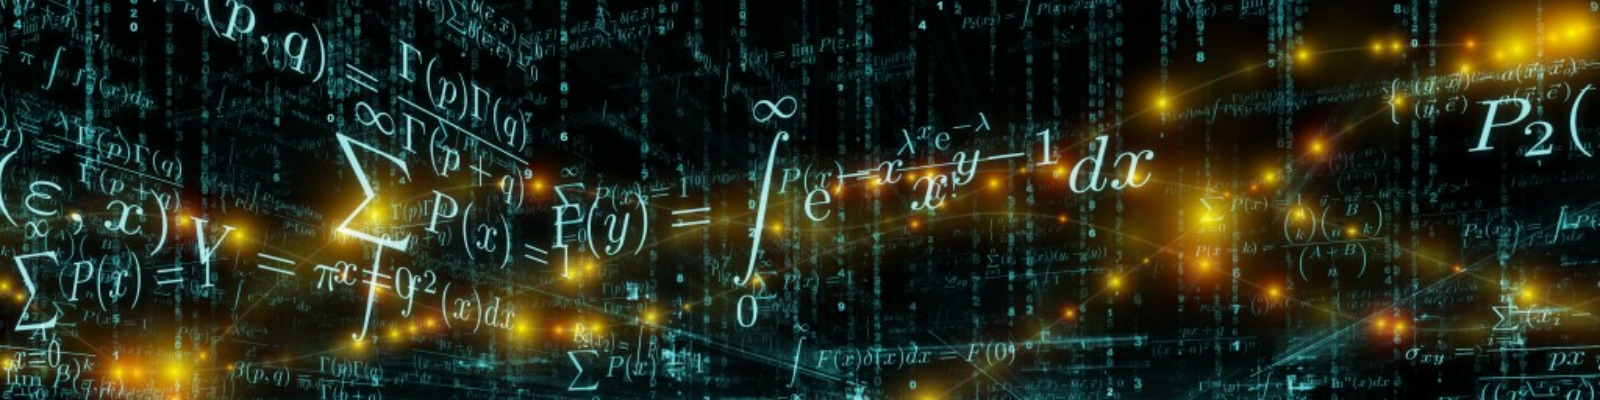
\includegraphics[scale=0.4]{banner.png}
    % \hskip-1.55cm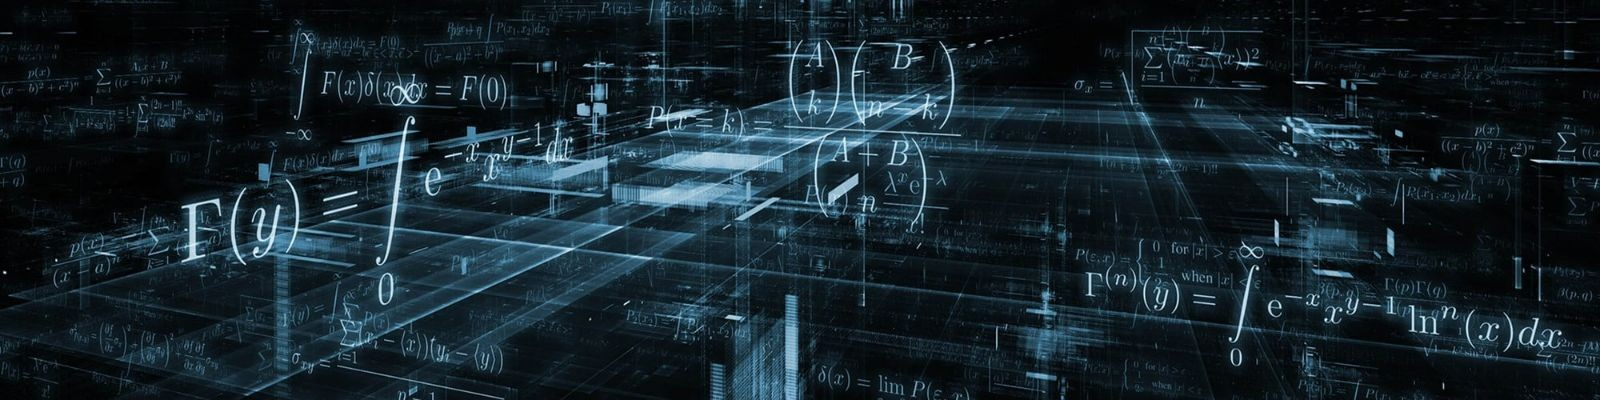
\includegraphics[scale=1.6]{banner4.jpg}
    \hskip-1.55cm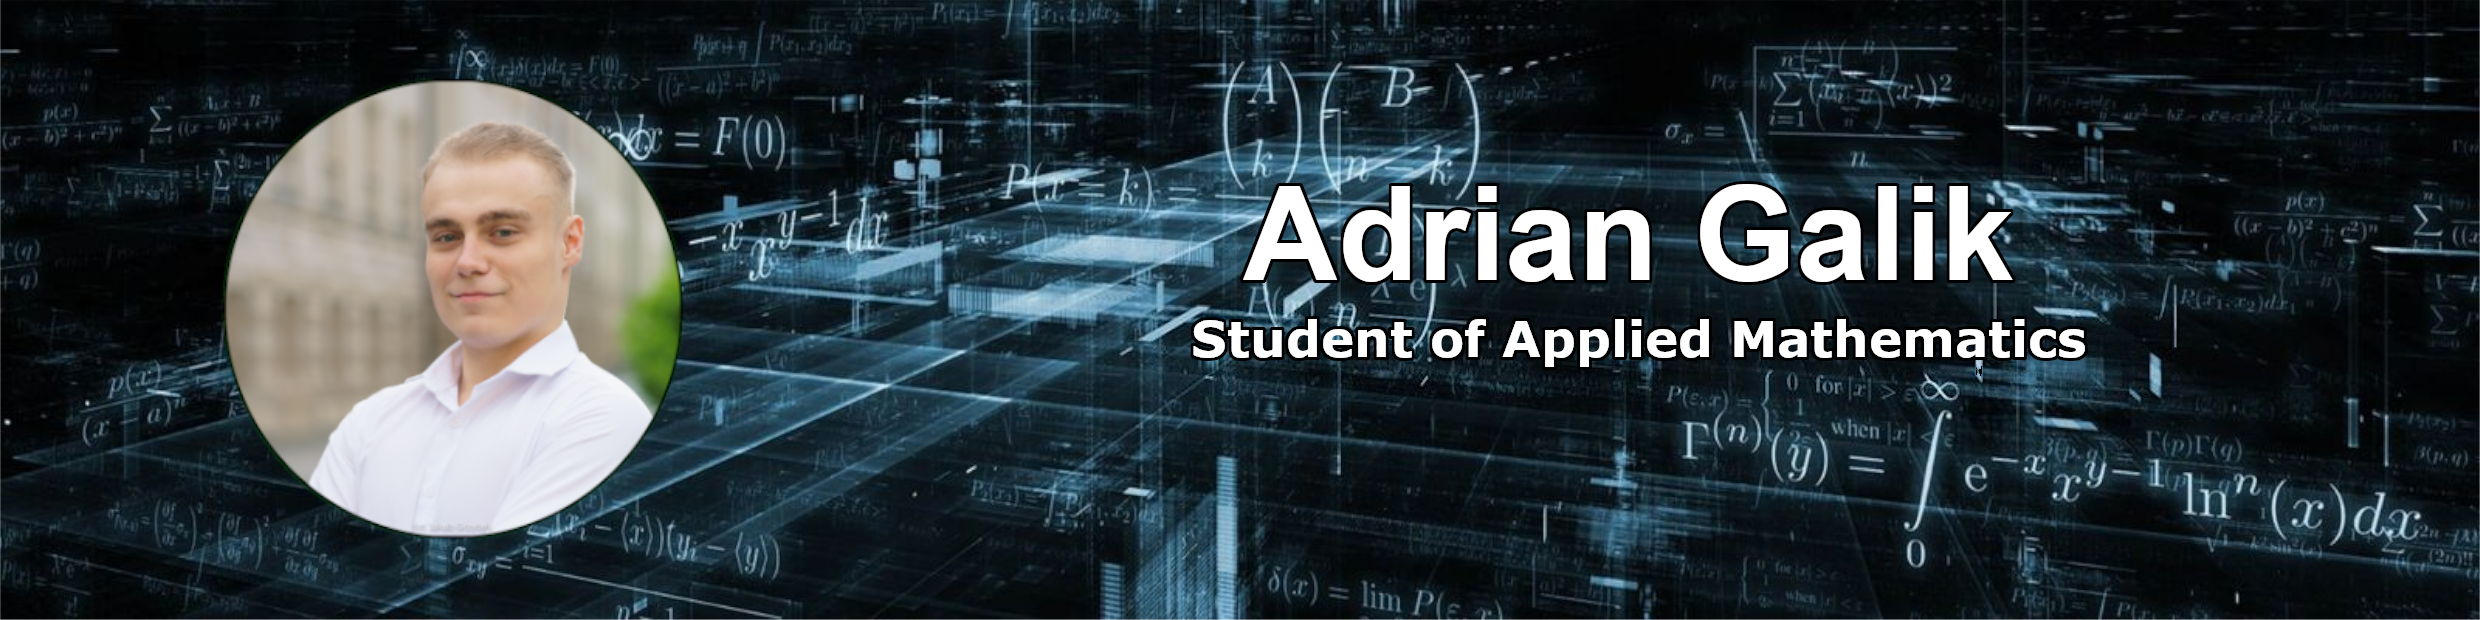
\includegraphics[scale=0.25]{benger_eng.png}
    % \hskip-1.55cm
\includegraphics[scale=1.6]{banner5.jpg}
    % \hskip-1.6cm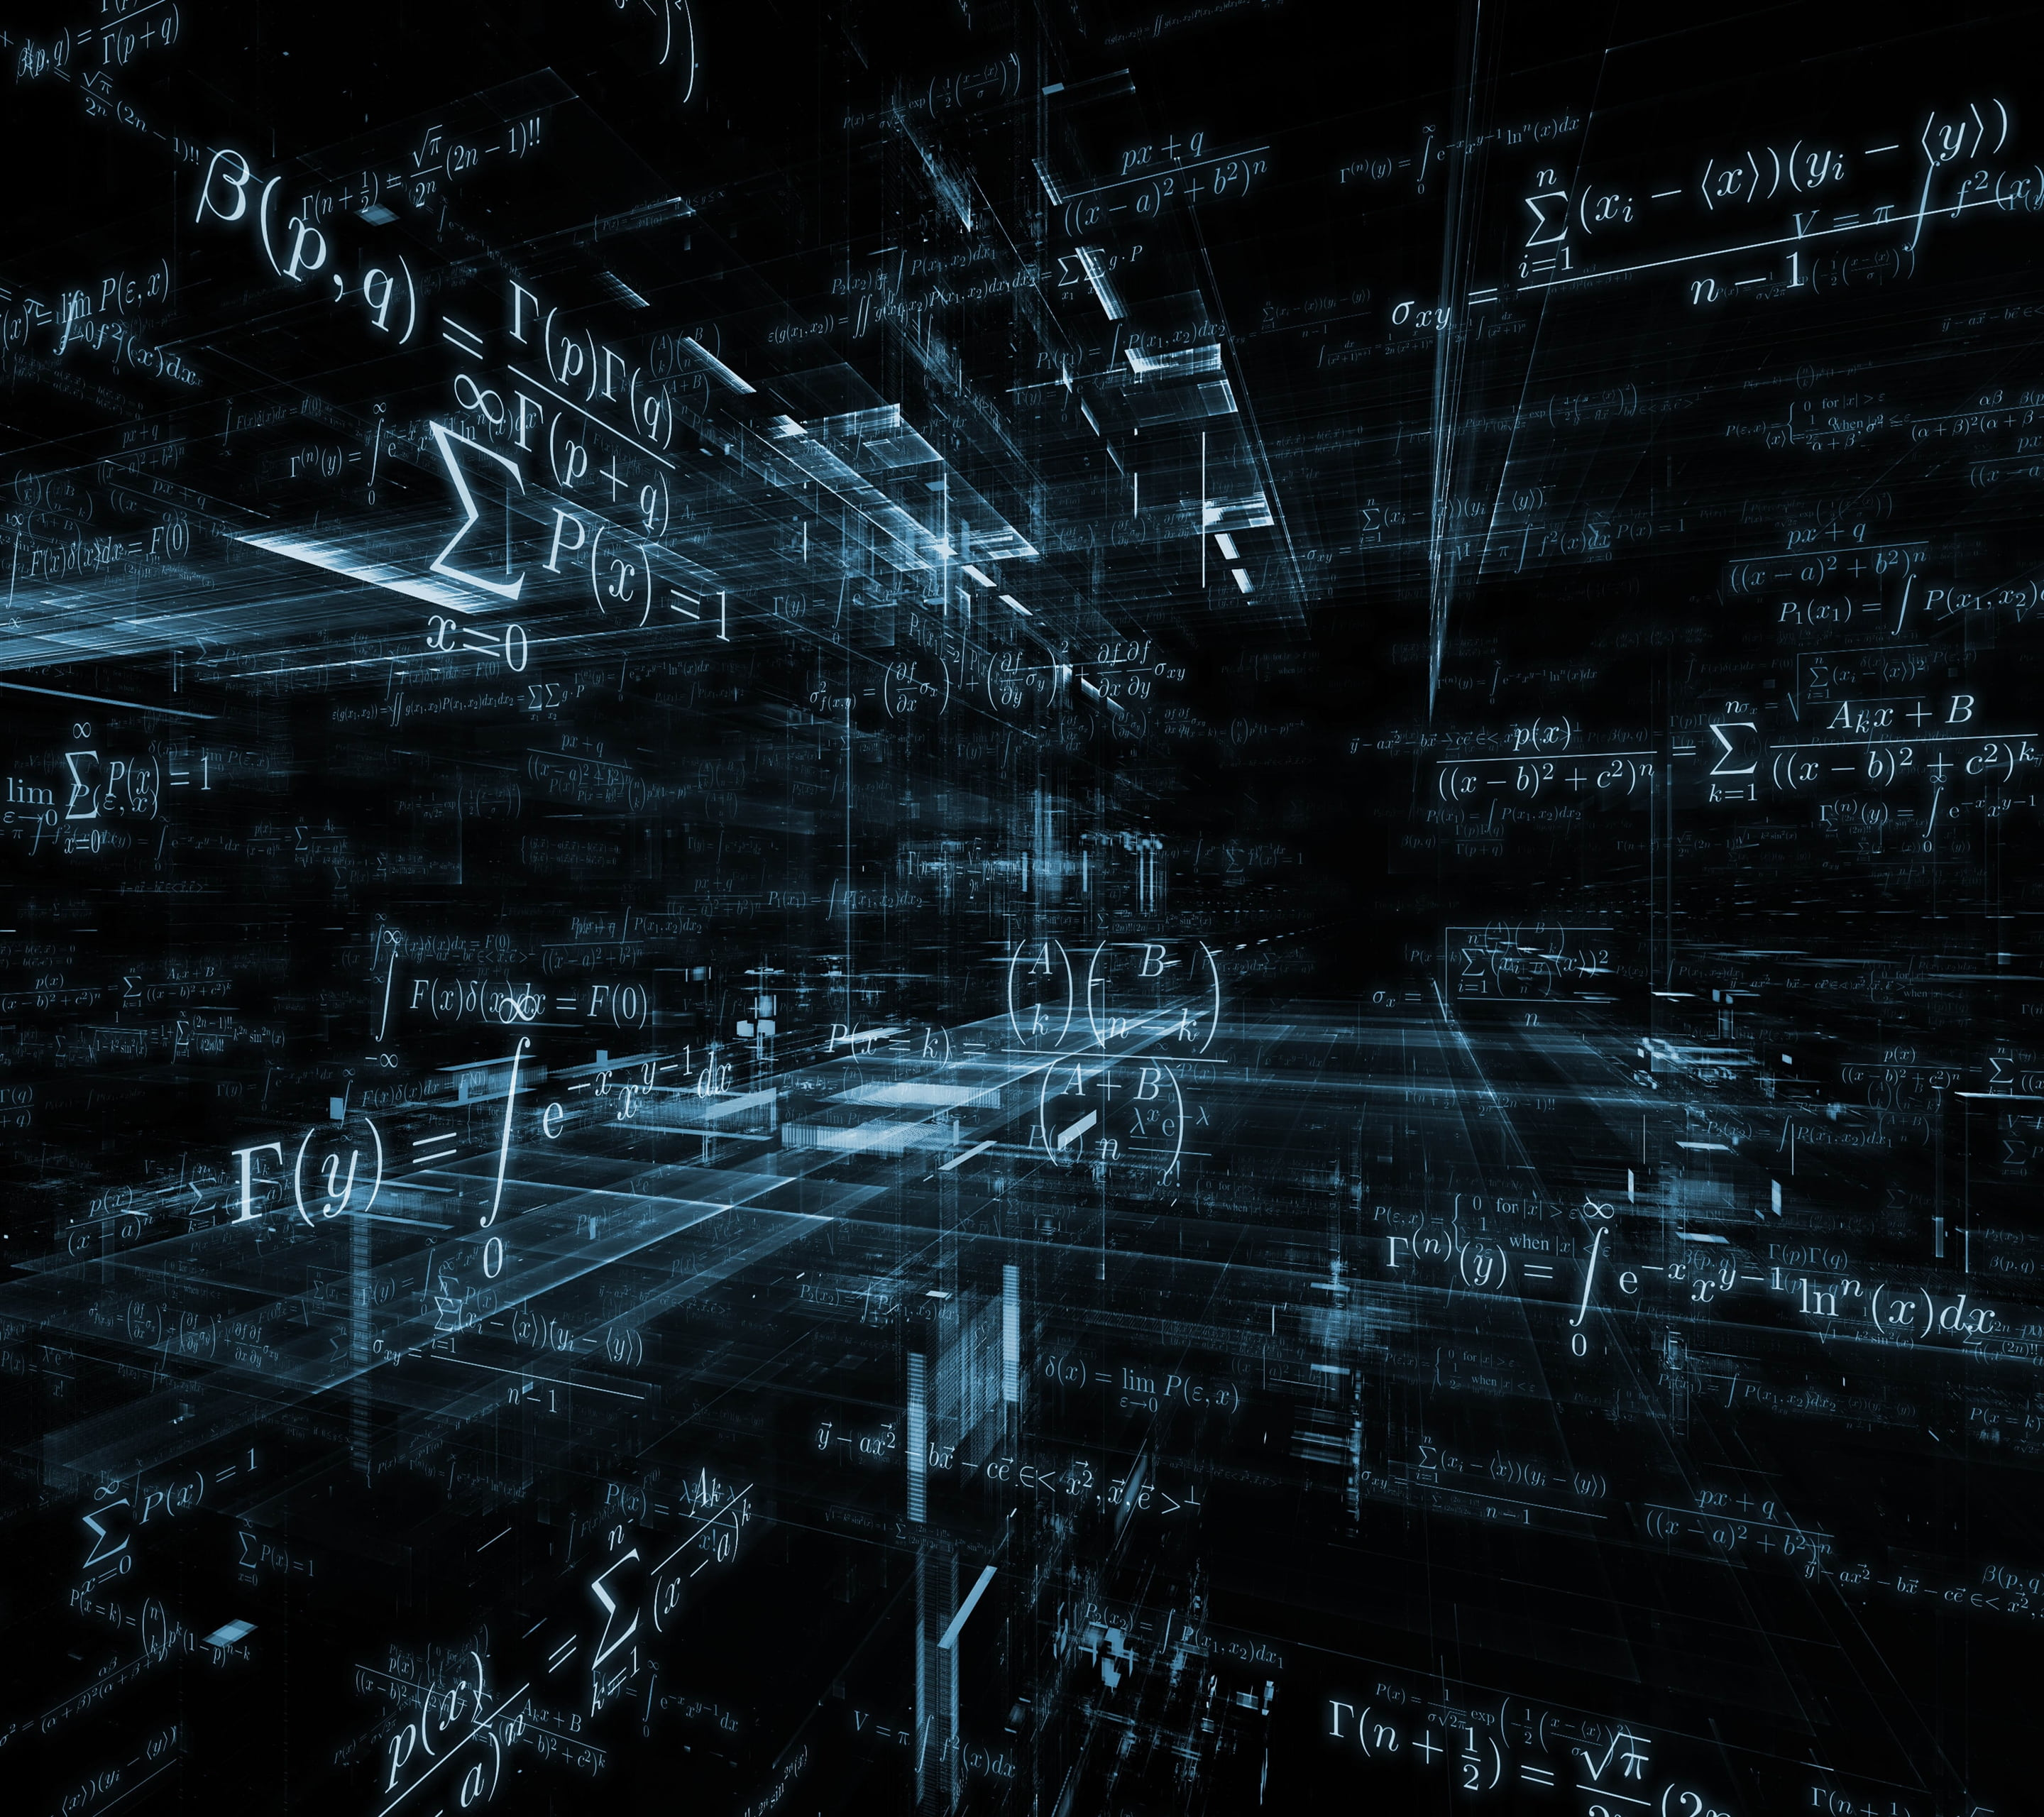
\includegraphics[height=0.20\textheight, width=1.5\textwidth]{banner2.jpg}
    % \hskip-1.6cm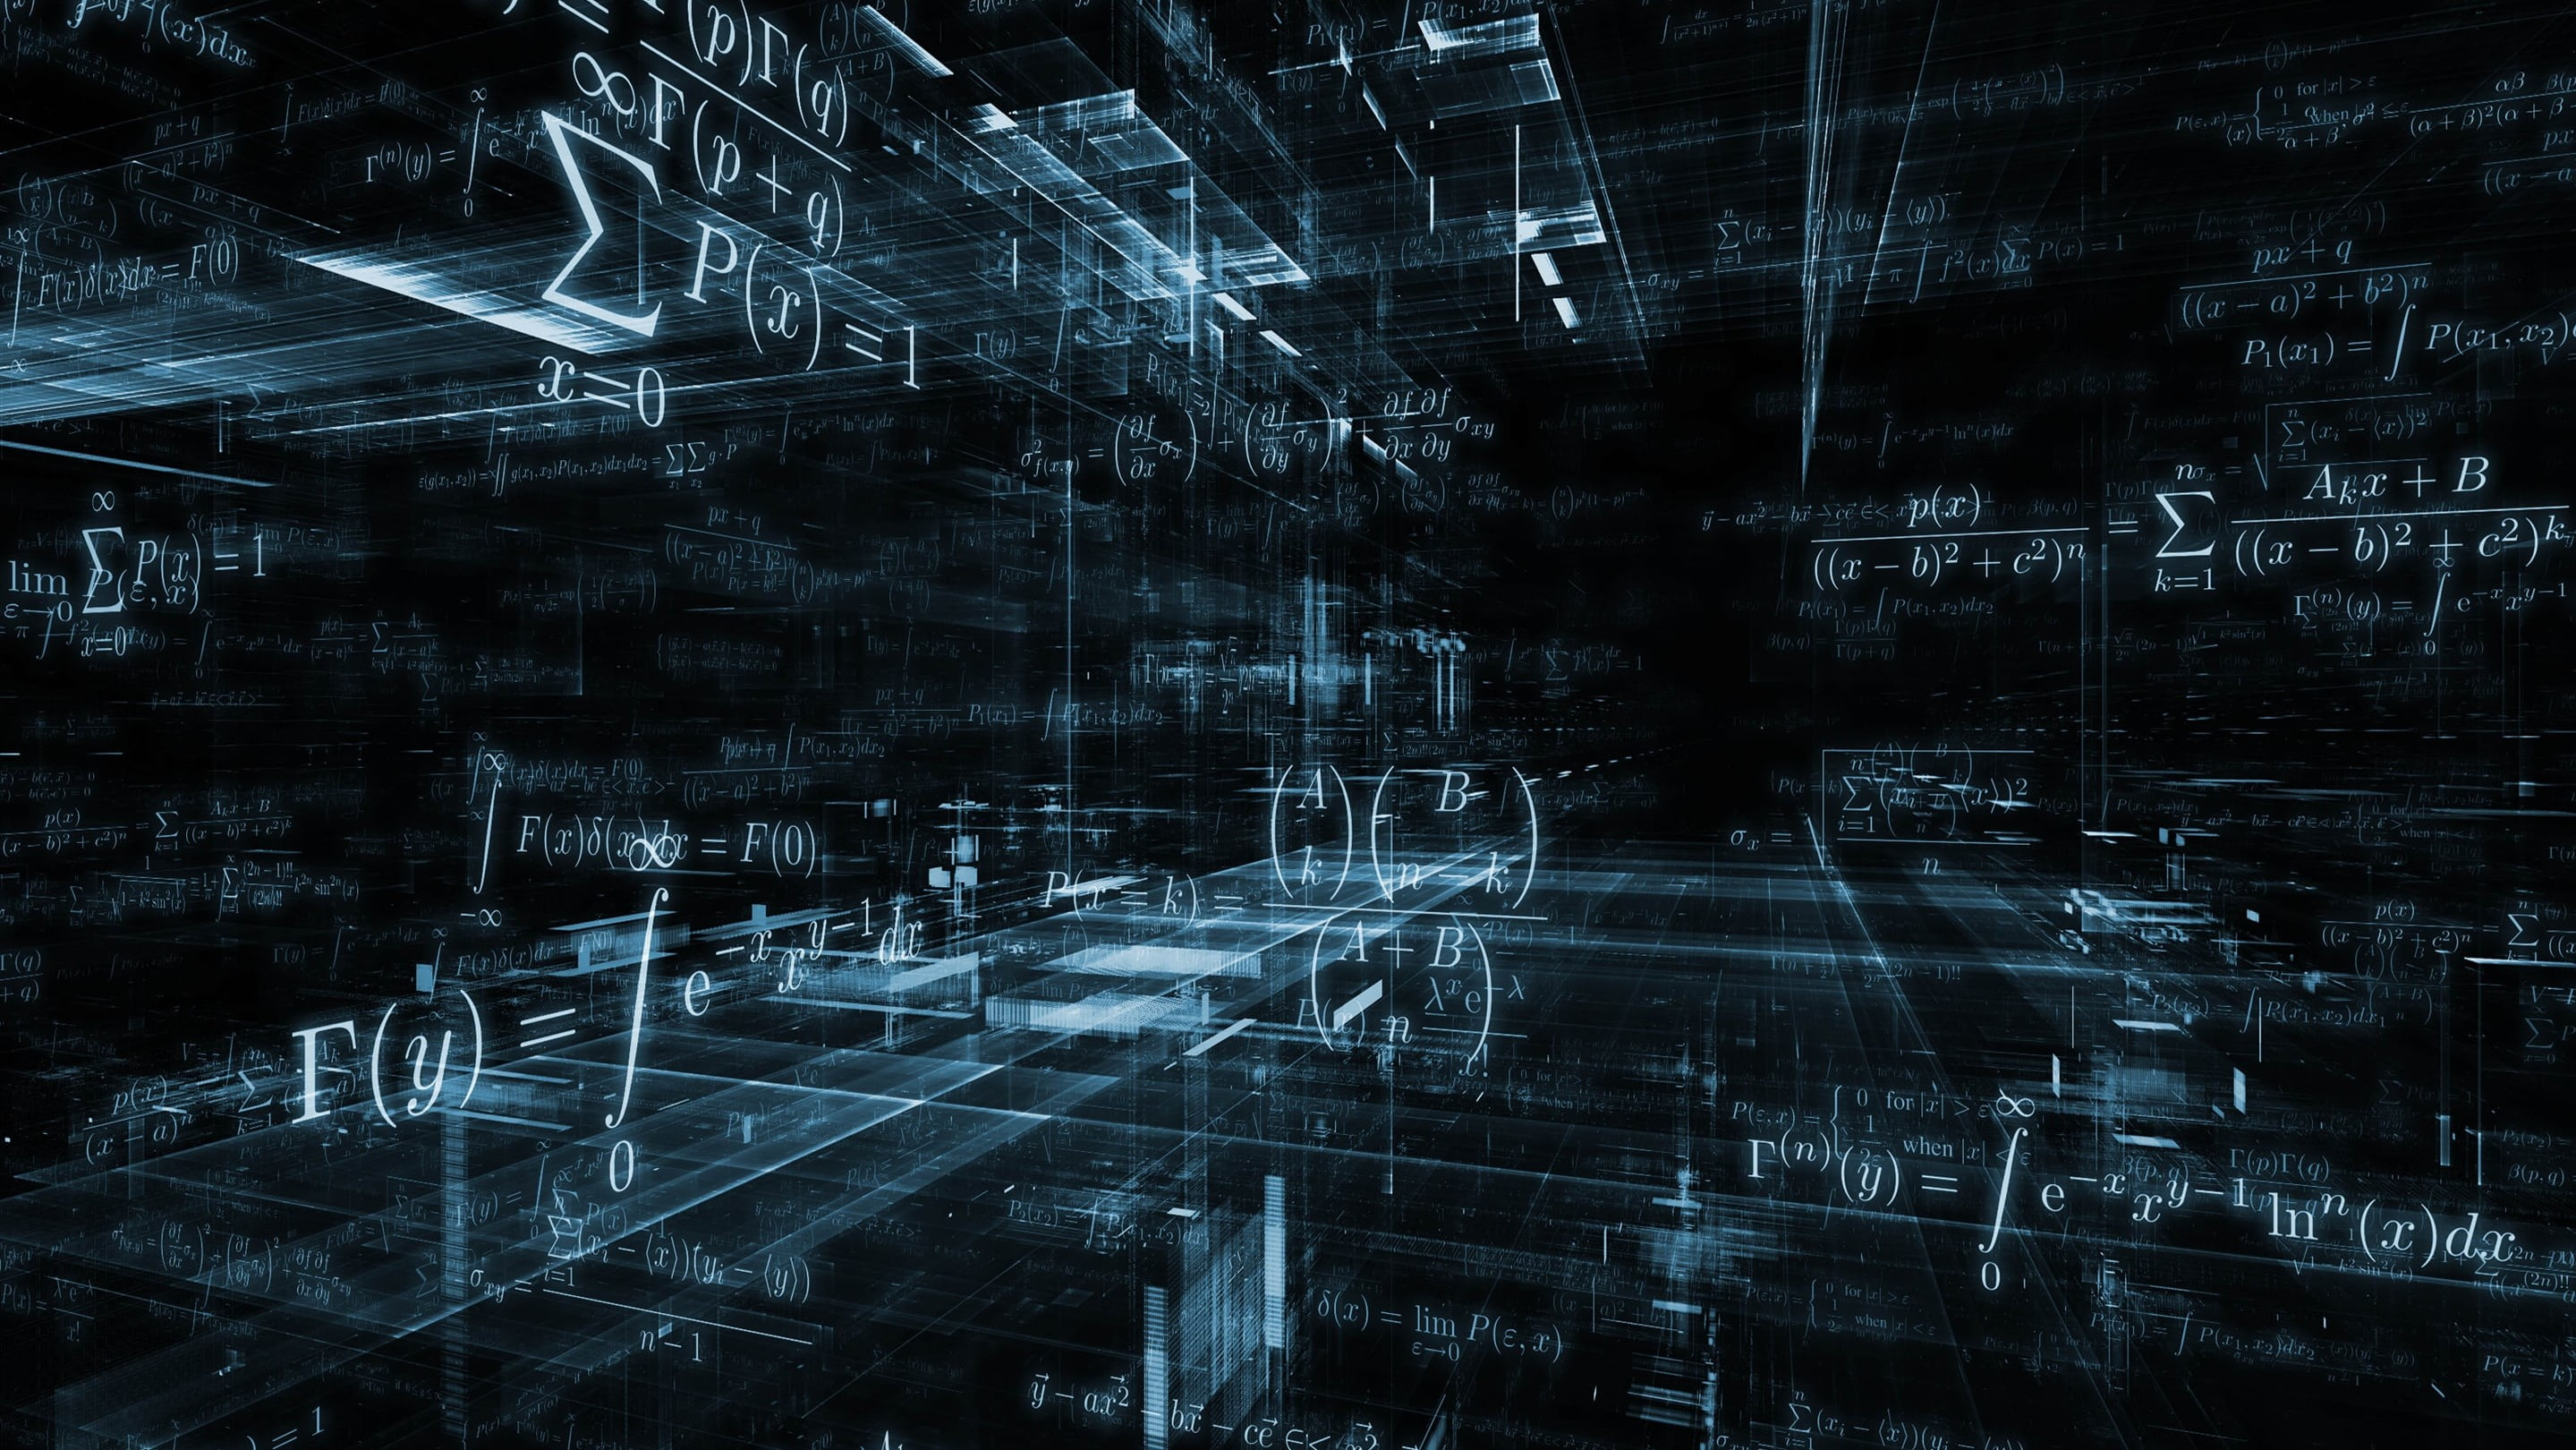
\includegraphics[height=0.25\textheight, width=1.5\textwidth]{banner3.jpg}
    \noindent
    \thispagestyle{empty}

    \vskip+0.4cm\begin{minipage}[t]{0.30\textwidth}
        \textbf{+48 663 383 000 \\
        adrian1galik@gmail.com} \\ \\
        \rule{6cm}{1pt} \\ \\
        \fontsize{14pt}{14pt}{\textbf{SKILLS:}}
        \fontsize{10pt}{10pt}
        \begin{itemize}[leftmargin=*]
            \setlength{\parskip}{0pt}
            % \setlength\itemsep{0pt} 
            \item \textbf{Python} intermediate level
            \item Abstract data structures: \textbf{Stacks, Queues, Trees, Graphs}
            \item Algorithmics
            \item Mathematical models and \\ statistical methods
            \item Applications of differential \\ equations
            \item Numerical calculations: \textbf{Julia}
            \item Network projecting and managing
            \item Data base managing: \textbf{SQL}
            \item Installation and operation of \\ computer systems: \textbf{Windows, \\ Linux}
            \item Creating and managing of \\ websites: \textbf{HTML, CSS, JavaScript, Flask, PHP}
            \item Text formatting language: \textbf{LaTeX}
            \item Distributed version control: \textbf{Git}
            \item Unix shell: \textbf{Bash} 
            \item Team work
        \end{itemize}
        \rule{6cm}{1pt} \\ \\
        \fontsize{14pt}{14pt}{\textbf{LANGUAGES:}}
        \fontsize{10pt}{10pt}
        \begin{itemize}[leftmargin=*]
            \setlength{\parskip}{0pt}
            % \setlength\itemsep{0pt} 
            \item Polish native
            \item English C1
        \end{itemize}
        \rule{6cm}{1pt} \\ \\
        \fontsize{14pt}{14pt}{\textbf{HOBBIES:}}
        \fontsize{10pt}{10pt}
        \begin{itemize}[leftmargin=*]
            \setlength{\parskip}{0pt}
            % \setlength\itemsep{0pt} 
            \item Astrophysics
            \item Mathematics
            \item Machine learning
        \end{itemize}
    \end{minipage}
    \hfill % horizontal space between columns
    \begin{minipage}[t]{0.60\textwidth}
        \fontsize{14pt}{14pt}{\textbf{ABOUT ME:}}
        \fontsize{10pt}{10pt} \\ \\
        Ambitious student of \textbf{Applayed Mathematics}. I'm using math \\ knowledge to write \textbf{algorithm} and to calculate astrophysics issues.
        My favourite programing language is \textbf{Python} and I would like to use it in my work. In the future, I see myself in the field of \textbf{machine learning}. \\ \\
        \rule{11cm}{1pt} \\ \\
        \fontsize{14pt}{14pt}{\textbf{EXPERIENCE:}}
        \fontsize{10pt}{10pt}
        \begin{itemize}[leftmargin=*]
            \setlength{\parskip}{0pt}
            % \setlength\itemsep{0pt} 
            \item Internship in firm \textbf{Sports Media}. Network and computer systems 
            \item Internship in firm \textbf{Zapaśnik IT}. Computer systems management
            \item Science club \textbf{Robocik}. Projecting artificial intelligence and creating \\ control algorithm  (\textbf{Python})
            \item Member of commite for Didactics and Student Rights
            \item Project simulating solar system (gravitational interactions) \\ by numerically solving the n-body problem  (\textbf{Python})
            \item Project numerically solving (without libraries) Friedman's differential equations defining the evolution of the universe.
            The goal was to obtain information about the universe, i.e. its age, past and future development (\textbf{Python})
        \end{itemize}
        \rule{11cm}{1pt} \\ \\
        \fontsize{14pt}{14pt}{\textbf{EDUCATION:}}
        \fontsize{10pt}{10pt}
        \begin{itemize}[leftmargin=*]
            \setlength{\parskip}{0pt}
            % \setlength\itemsep{0pt} 
            \item \textbf{Wrocław University of Science and Technology, Applied Mathematics, october 2021 - still}
            \item \textbf{Teleinformatics and Electronics School complex in Wrocław, \\ Technical school no. 7 (IT Technician), September 2017 - April 2021} 
        \end{itemize}
        \rule{11cm}{1pt} \\ \\
        \fontsize{14pt}{14pt}{\textbf{CERTIFICATIONS:}}
        \fontsize{10pt}{10pt}
        \begin{itemize}[leftmargin=*]
            \setlength{\parskip}{0pt}
            % \setlength\itemsep{0pt} 
            \item \textbf{Qualification EE.09 - Programming, creating and administering \\ websites and databases}
            \item \textbf{Qualification EE.08 - Installation and operation of computer systems, peripherals and networks}
        \end{itemize}
        \rule{0pt}{0pt} \\ \\ \\ \\ \\
        \fontsize{7pt}{5pt}\selectfont  
        I hereby give consent for my personal data included in my application to be processed for 
        the purposes of the recruitment process under the European Parliament's and Council of the 
        European Union Regulation on the Protection of Natural Persons as of 27 April 2016, with 
        regard to the processing of personal data and on the free movement of such data, and repealing 
        Directive 95/46/EC.
    \end{minipage}

\end{document}